%%%%%%%%%%%%%%%%%%%%%%%%%%%%%%%%%%%%%%%%%
% Beamer Presentation
% LaTeX Template
% Version 1.0 (10/11/12)
%
% This template has been downloaded from:
% http://www.LaTeXTemplates.com
%
% License:
% CC BY-NC-SA 3.0 (http://creativecommons.org/licenses/by-nc-sa/3.0/)
%
%%%%%%%%%%%%%%%%%%%%%%%%%%%%%%%%%%%%%%%%%

%----------------------------------------------------------------------------------------
%	PACKAGES AND THEMES
%----------------------------------------------------------------------------------------

\documentclass{beamer}

\mode<presentation> {
  \usetheme{Madrid}
}

\usepackage{graphicx}
\usepackage{booktabs}
\usepackage[utf8]{inputenc}

%------------------------------------------------------------------------------%
%                                  TITLE PAGE                                  %
%------------------------------------------------------------------------------%

\title[SWAP-IFC]{Secure Web Applications with Information Flow Control}

\author{Alexander Sjösten}
\institute[GU]
{
Master's Thesis in Computer Science \\
\medskip
Examiner: Andrei Sabelfeld 
}
\date{\today}

\begin{document}

\begin{frame}
\titlepage
\end{frame}

%------------------------------------------------------------------------------%
%                             PRESENTATION SLIDES                              %
%------------------------------------------------------------------------------%

\begin{frame}
  \frametitle{Security issues in web applications}
  
\end{frame}

%------------------------------------------------------------------------------%

\begin{frame}[fragile]
  \frametitle{JavaScript is bad!}
  Weak typing.
  \begin{block}{}
\begin{verbatim}
var age = prompt("What is your age?", "");
console.log(
    "You are now " + age + " years old. In 20 years you are " +
   (age + 20) + " years old!"
);
\end{verbatim}
  \end{block}
  What will the output be if 20 is the input??\pause \emph{"You are now 20 years old. In 20 years you are 2020 years old!"}
  \pause
  \newline
  Access to sensitive information (cookies, session tokens) in the browser. \pause
  
\end{frame}

%------------------------------------------------------------------------------%

\begin{frame}
  \frametitle{Tools used}
  JSFlow, a dynamic system for ensuring information flow control. \pause
  \newline
  JSFlow supports ECMA-262 v5, except for JSON and strict mode. \pause
  \newline
  \newline
  Haste, a compiler from Haskell to JavaScript. \pause
  \newline
  Ensures type safe JavaScript code. \pause
  \newline
  \newline
  Goal of the project is to extend Haste to produce JavaScript code targeting JSFlow.
\end{frame}

%------------------------------------------------------------------------------%


\begin{frame}
  \frametitle{Information flow control}
  Normally, applications in e.g. JavaScript has one input channel and one output channel.
  \begin{figure}[h]
    \includegraphics[scale=0.65]{images/flow_normal.eps}
  \end{figure}
  \pause
  Information flow control defines which flows are valid.
  \begin{figure}[h]
    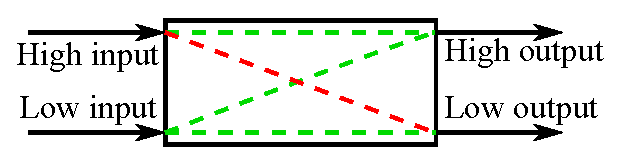
\includegraphics[scale=0.65]{images/flow_controlled.eps}
  \end{figure}
\end{frame}

%------------------------------------------------------------------------------%

\begin{frame}[fragile]
  \frametitle{Different flows}
  Two types of flows, \textbf{explicit} and \textbf{implicit} flows \pause
  \newline
  \begin{block}{Explicit flow}
\begin{verbatim}
  l := h;
\end{verbatim}
  \end{block}
  Private value is assigned \emph{directly} to a public variable.
  \pause
  \begin{block}{Implicit flow}
\begin{verbatim}
  h := h `mod` 2
  l := 0;
  if h == 1 then
      l := 1;
    else
      skip;
\end{verbatim}
  \end{block}
  Information of private values are leaked through \emph{indirectly} through e.g. control structures.
\end{frame}

%------------------------------------------------------------------------------%

\begin{frame}[fragile]
  \frametitle{Non-interference}
  Public output does not depend on private input. \pause

  \begin{block}{Function fullfilling non-interference}
\begin{verbatim}
f :: (Char, Int) -> (Char, Int)
f (c, i) = (chr (ord c + i), i + 42)
\end{verbatim}
  \end{block}
  \pause
  \begin{block}{Function not fullfilling non-interference}
\begin{verbatim}
f' :: (Char, Int) -> (Char, Int)
f' (c, i) = (c, ord c)
\end{verbatim}
  \end{block}
  \pause
  Information about the secret character (its ASCII value) is being leaked.
  \pause
  \newline
  However, a system satisfying non-interference is very strict...
\end{frame}

%------------------------------------------------------------------------------%

\begin{frame}
  \frametitle{Declassification}
  Sometimes it is necessary to release some private information.\pause
  \newline
  Imagine a login system. \pause
  \begin{itemize}
    \item User inserts username and password.
    \item Username is public data (i.e. low) and passwords are private data (i.e. high).
    \item If the username and password matches, the user is redirected.
    \item If the username and password does not match, message is shown to the user.
  \end{itemize}
  \pause
  If the system was non-interfered, no information would be given to the user.\pause
  \newline
  To solve this, declassification can be used.
\end{frame}

%------------------------------------------------------------------------------%

\begin{frame}[fragile]
  \frametitle{Examples of coding for JSFlow}
  Two important functions, \textbf{upg} and \textbf{declassify}.
  \pause
  \begin{block}{Upgrading a value}
\begin{verbatim}
  var l = 10;
  var h = upg(42);
\end{verbatim}
  \end{block}
  \textbf{l} will be a \emph{low} value, \textbf{h} will be a \emph{high} value.
  \pause
  \begin{block}{Upgrading a value}
\begin{verbatim}
  var h = upg(42);
  var l = declassify(h);
\end{verbatim}
  \end{block}
  \textbf{l} will be a \emph{low} value, containing the same value as \textbf{h}.
\end{frame}

%------------------------------------------------------------------------------%

\begin{frame}[fragile]
  \frametitle{SwapIFC - The library}
  \begin{itemize}
  \item Two different Monad, Applicative and Functor instances. \pause In particular, \textbf{return} differs:
\begin{verbatim}
#ifdef __HASTE__
  return = Flow . upg
#else
  return = Flow . return
#endif
\end{verbatim}
\pause
    \item Implementation of primitives for \textbf{Bool}, \textbf{Num}, \textbf{Frac}, \textbf{Ord} and \textbf{Eq} classes. \pause
\begin{verbatim}
Flow Low 10 .+. Flow Low 20 ==> Flow Low 30
\end{verbatim}
\pause
    \item Unsafe functions for \textbf{declassify} and \textbf{unwrap} a value. \pause
    \item Supports side effects using \textbf{IORef}.
  \end{itemize}
\end{frame}

%------------------------------------------------------------------------------%

\begin{frame}
  \frametitle{Side effects}
  
\end{frame}

%------------------------------------------------------------------------------%

\begin{frame}
  \frametitle{Integrating SwapIFC with Haste}
  
\end{frame}

%------------------------------------------------------------------------------%

\begin{frame}
  \frametitle{Communicating with JSFlow}
  
\end{frame}

%------------------------------------------------------------------------------%

\begin{frame}
  \frametitle{Demo!}
  \centering
  \Huge \textbf{DEMO!}
\end{frame}

%------------------------------------------------------------------------------%

\begin{frame}[fragile]
  \frametitle{Testing}
  \begin{itemize}
    \item Write the erroneous type signatures for each primitve. Compile error. \pause
\begin{verbatim}
  badFlow1 :: Num a
           => Flow High a
           -> Flow Low a
           -> Flow Low a
  badFlow1 = (.+.)
\end{verbatim}
\pause
    \item Unit testing. \pause
    \item Randomized testing with QuickCheck. \pause
      \begin{itemize}
        \item For every class (e.g. FlowNum), generate primitive and values. \pause
        \item Create flows using values. \pause
        \item Perform operation with values, check if correct. \pause
        \item Tag is only in type system. \pause Unsafe operations to the rescue! \pause
        \item Repeat 100000 times for every combination. \pause Result: No errors!
      \end{itemize}
  \end{itemize}
\end{frame}

%------------------------------------------------------------------------------%

\begin{frame}
  \frametitle{Conclussion}
  \begin{itemize}
    \item Library for static information flow control. \pause
    \item Non-interference is guaranteed if no unsafe operations are used. \pause
    \item Generates valid code for JSFlow w.r.t. low flows. \pause
    \item Can handle side effects.
  \end{itemize}
\end{frame}

%------------------------------------------------------------------------------%

\begin{frame}
  \frametitle{Future work}
  As with everything, nothing is perfect. \pause
  \begin{itemize}
    \item Implement full support for JSFlow (i.e. support High flows) and test the code generation. \pause
    \item Add support for Haste.App. \pause
    \item End-to-end communication, including database. \pause
    \item More features for JSFlow, including JSON and browser support. \pause
    \item More primitives for SwapIFC.
  \end{itemize}
\end{frame}

%------------------------------------------------------------------------------%

\begin{frame}
  \frametitle{The end!}
  \Huge
  \begin{center}
    Thank you!
  \end{center}
  \begin{center}
    Questions?
  \end{center}
\end{frame}

%------------------------------------------------------------------------------%

\end{document} 
